%% Copyright (c) 2003,2004,2005  INRIA Sophia-Antipolis (France).
%% All rights reserved.
%%
%% This file is part of CGAL (www.cgal.org).
%% You can redistribute it and/or modify it under the terms of the GNU
%% General Public License as published by the Free Software Foundation,
%% either version 3 of the License, or (at your option) any later version.
%%
%% Licensees holding a valid commercial license may use this file in
%% accordance with the commercial license agreement provided with the software.
%%
%% This file is provided AS IS with NO WARRANTY OF ANY KIND, INCLUDING THE
%% WARRANTY OF DESIGN, MERCHANTABILITY AND FITNESS FOR A PARTICULAR PURPOSE.
%%
%% $URL$
%% $Id$
%% 
%%
%% Author(s)     : Menelaos Karavelas <mkaravel@iacm.forth.gr>



\begin{ccRefConcept}{SegmentDelaunayGraphDataStructure_2}

%% \ccHtmlCrossLink{}     %% add further rules for cross referencing links
%% \ccHtmlIndexC[concept]{} %% add further index entries
\ccCreationVariable{sdgds}
\ccDefinition

The concept \ccc{SegmentDelaunayGraphDataStructure_2} refines the
concept \ccc{ApolloniusGraphDataStructure_2}. In addition
it provides two methods for the merging of two vertices joined by an
edge of the data structure, and the splitting of a vertex into two.
The method that merges two vertices, called \ccc{join_vertices}
identifies the two vertices and deletes their common two faces. The
method that splits a vertex, called \ccc{split_vertex} introduces a
new vertex that shares an edge and two faces with the old vertex (see
figure below). Notice that the \ccc{join_vertices} and
\ccc{split_vertex} operations are complementary, in the sense that one
reverses the action of the other.

\begin{figure}[htb]\label{fig-sdgds-split-join}
\begin{ccTexOnly}
\begin{center}
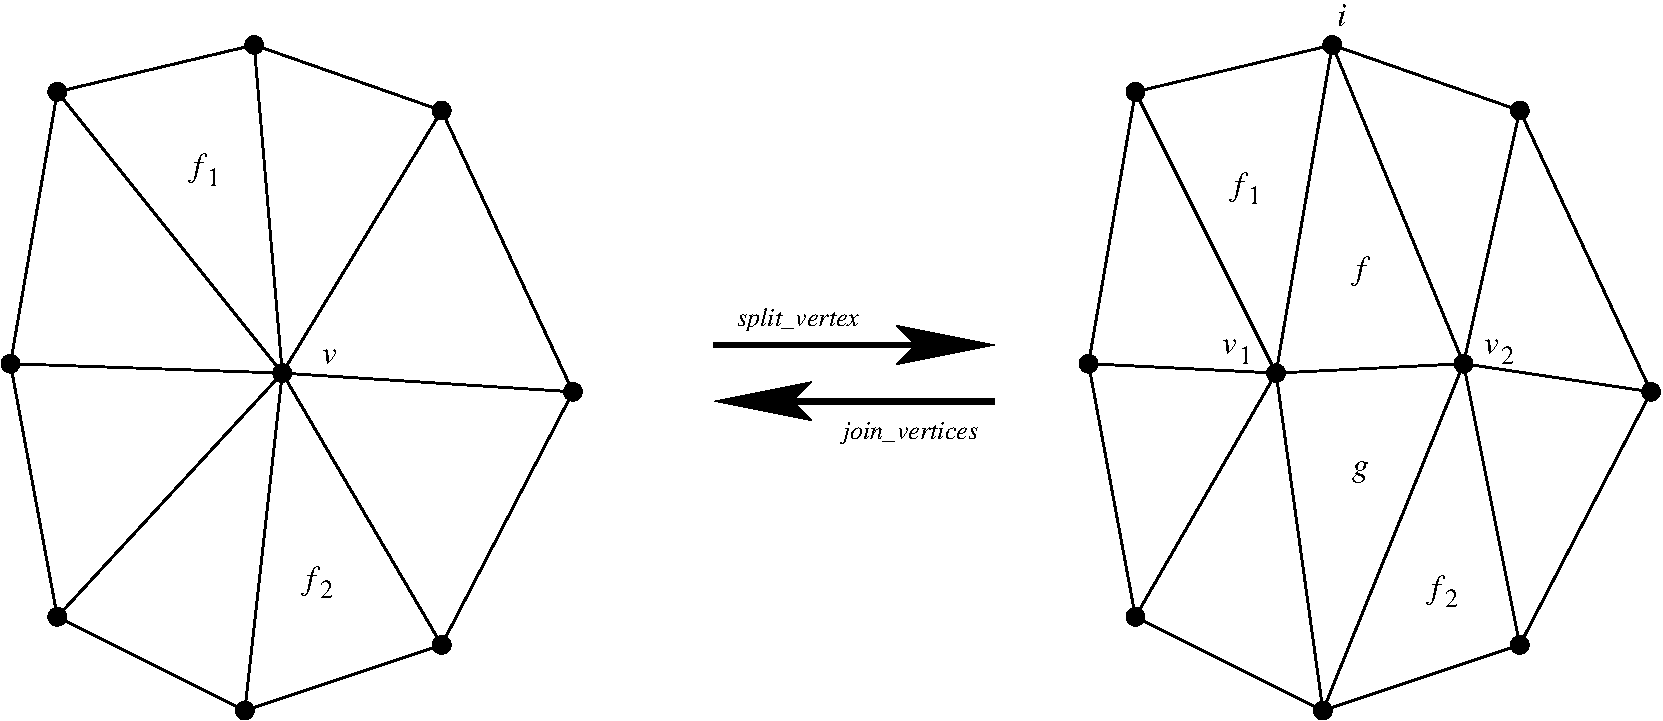
\includegraphics[width=0.95\textwidth]
{Segment_Delaunay_graph_2_ref/sdg-join_split}
\end{center}
\end{ccTexOnly}
\begin{ccHtmlOnly}
<center>
<img border=0 src="./sdg-join_split.gif" align=middle
alt="The join and split operations''
title="The join and split operations">
</center>
\end{ccHtmlOnly}
\begin{ccHtmlOnly}
<br><font size=-1>
\end{ccHtmlOnly}
\caption{The join and split operations. Left to right:
The vertex \ccc{v} is split into $v_1$ and $v_2$. The faces $f$ and
$g$ are inserted after $f_1$ and $f_2$, respectively, in the
counter-clockwise sense. The vertices $v_1$, $v_2$ and the faces $f$
and $g$ are returned as a \ccc{boost} \ccc{tuple} in that order.
Right to left: The edge \ccc{(f,i)} is collapsed, and thus the
vertices $v_1$ and $v_2$ are joined. The vertex \ccc{v} is
returned.}
\begin{ccHtmlOnly}
</font>
\end{ccHtmlOnly}
\end{figure}



We only describe the additional requirements with respect to the
\ccc{ApolloniusGraphDataStructure_2} concept.

\ccRefines
\ccc{ApolloniusGraphDataStructure_2}

\ccHeading{Modification}
\ccThree{Vertex_handle}{sdgds.join_vertices(Face_handle v, int i)+}{}
%
\ccMethod{Vertex_handle join_vertices(Face_handle f, int i);}{Joins
  the vertices that are endpoints of the edge \ccc{(f,i)}. It returns
  a vertex handle to common vertex.}
\ccGlue
\ccMethod{boost::tuples::tuple<Vertex_handle, Vertex_handle, Face_handle,
Face_handle>
  split_vertex(Vertex_handle v, Face_handle f1, Face_handle
  f2);}{Splits the vertex \ccc{v} into two vertices \ccc{v1} and
  \ccc{v2}. The common faces \ccc{f} and \ccc{g} of \ccc{v1} and
  \ccc{v2} are created after (in the counter-clockwise sense) the
  faces \ccc{f1} and \ccc{f2}. The 4-tuple \ccc{(v1,v2,f,g)} is
  returned (see Fig. \ref{fig-sdgds-split-join}).}

\ccHasModels
\ccc{CGAL::Triangulation_data_structure_2<Vb,Fb>}

\ccSeeAlso
\ccc{TriangulationDataStructure_2}\\
\ccc{ApolloniusGraphDataStructure_2}\\
\ccc{SegmentDelaunayGraphVertexBase_2}\\
\ccc{TriangulationFaceBase_2}

\end{ccRefConcept}

% +------------------------------------------------------------------------+
%%RefPage: end of main body, begin of footer
% EOF
% +------------------------------------------------------------------------+
